\section{Recognize the Page Title}
\label{sec:title}

The title of a web page (string enclosed in {\tt<title>} tag)
helps us identify a ``top-$k$'' page.
There are several reasons for us to utilize the page title to recognized a ``top-$k$'' page.
First, for most cases, page titles serve to introduce the topic of the main body.
Second, compared to the complex and various form of page body,
page titles are simpler as they are all plain text.
Last but not least, as for time, title analysis is much less expensive than the rest parts of the system,
thus, if the title analysis indicates that a page is not a ``top-$k$'' page,
we can avoid wasting time on parsing and analyzing the page body.
The last point is especially precious
as the system is going to process massive web pages.

\begin{figure}
\centering
\epsfig{file=pics/PageTitle.eps,width=0.6\columnwidth}
\caption{A Sample Top-K Like Title}
\label{fig:title}
\end{figure}

In the following discussion, we define titles that is likely to be a title of a ``top-$k$'' page as ``top-$k$ like'' titles.
In general,
a ``top-$k$ like'' title represents the topic of a ``top-$k$'' list.
Figure \ref{fig:title} shows a typical ``top-$k$ like'' title.
Note that a ``top-$k$ like'' title may contain multiple segments, and
usually only one segment describes the topic or concept of the list.
In addition to the list number $k$(e.g, 20) and the head concept(e.g, ``scientists'') we mentioned in \ref{sec:intro},
a ``top-$k$ like'' title could include some other elements, such as the criteria (e.g, ``most influential'')
and qualifiers (e.g, ``alive today'').

The goal of the classifier is to recognize ``top-$k$ like'' titles.
Furthermore,
the classifier also outputs the list size $k$ as well as
% transfers the cardinal digit word
%(word like ``ten'' or ``fifteen'') into the number $k$,
a set of Probase concepts which are mentioned in the title.

To build the classifier, we trained a Conditional Random Field (CRF) \cite{CRFLafferty} model
from 4000 negative titles (titles that contain a number but
are not actually ``top-$k$ like'') and 2000 positives titles. The number $k$
is especially important because it serves as an anchor to a phrase that
represent a ``top-$k$ like'' concept or topic.
We use \textit{word, lemma,} and \textit{POS tag} \cite{StanfordParser}
as the basic feature set.

However, just like other natural language task, the classifier cannot be 100\% correct.
What is worse, some pages with a ``top-$k$ like'' title actually do not contain ``top-$k$'' list
(that is why we just call them ``top-$k$ like'' titles rather than ``top-$k$'' titles).
A typical case is slide-show pages , such as the page\cite{TopFootball} in Figure \ref{fig:slideshow}.
Although these pages are also about ``top-$k$'' lists,
they present it in a page chain that each page only contain one list item.
For false positives (i.e, pages that are wrongly recognized as ``top-$k$'' pages)
we may still filter them in the later list extraction part.
But on the contrary, we are helpless for false negatives (i.e, ``top-$k$'' pages that are wrongly filtered).
Therefore when we design the classifier, we give priority to the recall performance.

\begin{figure}
\centering
\epsfig{file=pics/page4.eps,width=0.9\columnwidth}
\caption{A slide-show page snapshot\cite{TopFootball}}
\label{fig:slideshow}
\end{figure}

\subsection{Collect Training Data}
In order to build a practical model, a large training data set with abundant positive and negative cases is necessary.
As we have mentioned, to build the CRF model, we used a set of 2000 positive titles and 4000 negative ones as the training data.
However, it is quite challenging to generate the training data considering the fact that the project is short
of both labor force and time. Actually, the challenge mainly lies in collecting the positive ``top-$k$ like'' titles. As we estimated in Section \ref{sec:topKSum}, the ``top-$k$'' pages account for about 1.4\textperthousand~
of total web pages. Although the absolute number of ``top-$k$'' pages is still very large (over 2 million),
we may need to go through millions web pages for 2000 ``top-$k$ like'' titles.

In order to narrow the target, we can focus on the titles with at least one number. However, in English titles, numbers can be either digits like
``10'' or cardinal numeral like ``ten''. To handle both the forms, we use Stanford Parser\cite{StanfordParser} to label the POS tag for each word in the title. Stanford Parser will label numbers with the uniform tag ``CD'' (see Table \ref{tab:tagSet}). Finally ,we grab about 8 million titles with numbers from $1/10$ of the whole web. But ``top-$k$ like'' titles are still too sparse among those titles.
In Section \ref{sec:evalTitle}, we randomly sampled 2000 titles with numbers and only find 50 ``top-$k$ like'' titles. As a result, we need to sample over 80,000 titles to get 2000 ``top-$k$ like'' titles, which are still too many for us.

From observation, we find several very strong positive rules, which is listed as follows.
\begin{enumerate}
  \item \textbf{``top CD''}:
  If a title contains the word ``top'' and the word is followed by a number, it is a ``top-$k$ like'' title. For example, ``top 10 NBA players who could be successful general managers''.
  \item \textbf{``CD JJS''}:
  According to Table \ref{tab:tagSet}, ``JJS'' stands for a superlative adjective. Thus a title that contains a number followed  by a superlative adjective is a ``top-$k$ like'' title. For example, ``20 highest buildings in China''.
  \item \textbf{``CD RBS JJ''}:
   According to Table \ref{tab:tagSet},
   ``RBS'' and ``JJ'' stands for a superlative adverb and an adjective respectively. If a title contains a sequence of a number, a superlative adverb and an adjective, it is a ``top-$k$ like'' title. For example, ``5 most expensive watches in the world''.
\end{enumerate}

We can directly build a classifier based on the three rules. About this rule-based classifier, there is good news and bad news.
The good news is that the precision of the classifier is very high. The bad news is that there are still many ``top-$k$ like'' titles that do not satisfy the three rules, such as ``10 movies that you should not miss''. In fact, these rules can only cover half of all the ``top-$k$ like'' titles, in other words, the recall is only 50\%.
Since we put the recall performance of the title classifier in the first place, this rule-based approach is not completely qualified.
But at least, these rules solve half of the problem, so now we can focus on the left ``top-$k$ like'' titles.

The true reason that we meet such a bottleneck is that we make an unnecessary assumption, that the titles in the training data set must be titles of real web pages. Instead of collecting titles of ``top-$k$'' pages, we can just ``make up'' these titles, which is much easier.
In fact, we can automatically generate ``top-$k$ like'' titles that satisfy none of the rules above from the ``top-$k$ like'' titles that satisfy the first rule, according to the following observation.

\begin{itemize}
  \item \textbf{Observation}: For a title that satisfy the rule ``top CD'', it will not harm the original meaning to remove the word ``top''.
\end{itemize}

This observation is true for most cases, e.g., for the title ``top 10 NBA players who could be successful general managers'', we can delete the ``top'' and it becomes ``10 NBA players who could be successful general managers'', which is still a ``top-$k$ like'' title.

With this method, we can generate the 4000 positive cases in a full automatical manner: first we obtain 2000 titles using the ``top CD'' rule; then we remove the ``top'' in each title and get 2000 new titles. Combined with 2000 negative cases, we finally have a large enough training data set.

\subsection{Design the Model Pattern}
With the training data set, we would like to use the tool CRF++\cite{crfppHome} to generate the classifier model.
Before we do that, we have to design the model pattern first. The model pattern is the input format for CRF++ to learn or test data,
including used features, meaning of tokens, set of answer tags and so on. Figure \ref{fig:crfpp}(a) shows a sample model pattern.

After numerous attempts and experiments, we decide the model pattern as a 9-gram centering on a number word. Table \ref{tab:modelPattern} shows the model pattern of the title in Figure \ref{fig:title}.
We list a few steps as follows to generate this model pattern from a title and discuss the reason we adapt this pattern.

\begin{enumerate}
  \item \textbf{Split the title}:

  As we can see in Figure \ref{fig:title}, a web page title may consist of multiple segments, which is separated by splitters like ``-'', ``$|$'' or ``:''. Among these segments, only the main segment (e.g, Segment 1 in Figure \ref{fig:title}) will tell us the topic of the page, while other segments show additional information such as the website name, which is not of the interest. Therefore, we can split the title and only keep those segments with a number (since we cannot tell which one is the main segment).
  \item \textbf{Generate the features}:

  As is shown in Table \ref{tab:modelPattern}, we select four kinds of features: word itself, lemma, POS tag and concept value.

  Lemma and POS tags can be generated by Stanford Parser\cite{StanfordParser}, as we have mentioned in Section \ref{sec:stanfordParser}.  In that section, we also mention some higher-level parsing results that are also available, such as Stanford dependencies and the phrase structure tree. However, there are some reasons that we fail to integrate them into our model pattern. First, Stanford dependencies and the phrase structure tree are semantic features, which are corresponding to sentences; while lemma and POS tags are corresponding to words. As the token of the model pattern is a word, we can hardly transfer the semantic features to a word-wise feature.
  Second, since the parser is originally designed from normal text, the higher-level parsing results are not very accurate for web page titles.
  Third, it will take much more time to parse the Stanford dependencies and the phrase structure tree than to get the POS tags and lemma.

  The concept value indicates whether the corresponding word and word phrases are concepts in Probase\cite{WuLWZ12:Probase}. In a concept value, the $i$th bit will be 1 if the $i$-gram that ends with the word is an Probase concept, especially the first bit is the case for the word itself.
  For example, in Table \ref{tab:modelPattern}, the concept value for ``scientists'' is 3, which means both ``scientist'' and ``influential scientist'' are Probase concepts. Not only does the concept value play an important role in the model, but also is it helpful for us to obtain the concept list of the title.
  \item \textbf{Generate the 9-gram}:

  Unlike other model pattern that use the whole sentences, our model pattern cut out a fixed-length word sequence: the number, four words before it and four words after it. Here we give some reasons. The number k is especially important because it serves as an anchor to a phrase that represent a ��top-$k$ like�� concept or topic, in other words, the ``9-gram window'' is sufficient to make a correct judgement. Second, we can transfer the original task, which is to recognize ``top-$k$'' title, into a task to recognize the a proper number k with proper context, which is much easier and more suitable for CRF learning. Last but not the least, we can realize automatic labeling for training data: we only label the number that satisfy the rule ``top CD'' as ``TRUE'',otherwise ``FALSE''. If we use the whole sentence as the model pattern, we have to manually solve the number ambiguity in the titles that contain multiple numbers.

  As a special case, if there are no enough words before or after the number, we just fill up the vacancies  with null token, just like the case in Table \ref{tab:modelPattern}.
\end{enumerate}

Using the pattern above, we successfully trained a CRF model with the training data and then build the outside title classifier.

\begin{table}
\centering
\caption{A sample model pattern}
\begin{tabular}{|l|l|l|l|l|}
\hline
\textbf{word}    &\textbf{lemma}   &\textbf{POS}    &\textbf{concept}   &\textbf{tag} \\ \hline
NULL	&NULL  &NULL	&NULL  &FALSE\\
NULL	&NULL  &NULL	&NULL  &FALSE\\
NULL	&NULL  &NULL	&NULL  &FALSE\\
NULL	&NULL  &NULL	&NULL  &FALSE\\
20	&20  &CD	&0  &TRUE\\
most	&much  &RBS	&0 &FALSE\\
influential	&influential    &JJ	&0  &FALSE\\
scientists	&scientist   &NNS	&3 &FALSE\\
alive	&alive    &JJ	&0  &FALSE\\
\hline
\end{tabular}

\label{tab:modelPattern}
\end{table}

\subsection{Build the title classifier}


\begin{figure}
\centering
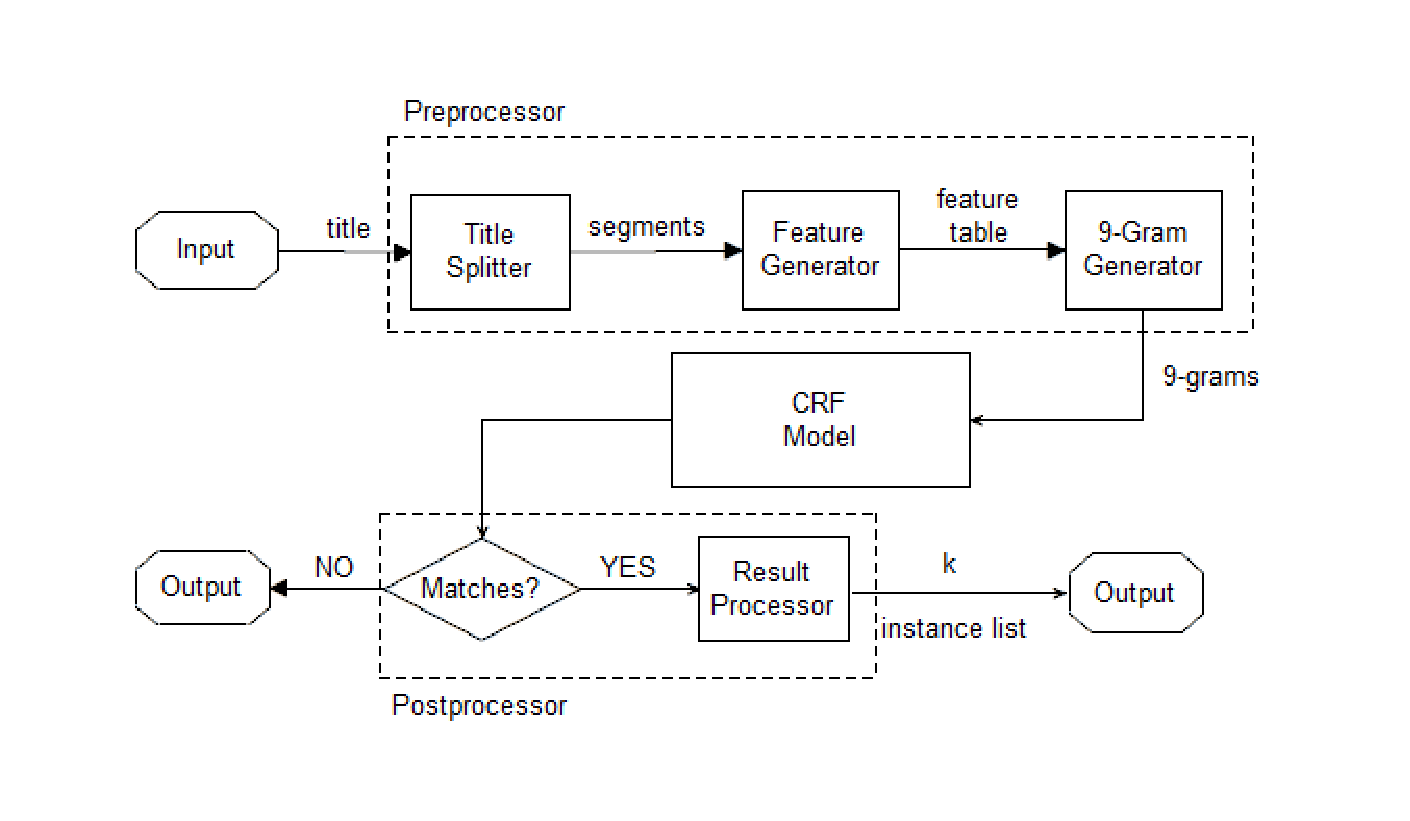
\epsfig{file=pics/TitleClassifier.eps,width=0.9\columnwidth}
\caption{The flow chart of the title classifier}
\label{fig:titleClassifier}
\end{figure}

As is shown in Figure \ref{fig:titleClassifier},
the classifier centers on the model. It consists of three parts: the preprocessor, the model and the postprocessor.

The preprocessor is very similar to the steps in generating the model pattern, since the test input should also follow the format.
The only difference is that before the title splitter, we need to filter ill-formatted writing in the title and lowercase all the words,
in order to optimize the performance of Stanford Parser.

The model will attach an additional column to the input 9-gram as the answer tag. The answer tag is either ``TRUE'' or ``FALSE''.
We are only interested in the 5th tag, which indicates whether this title is a ``top-$k$ like'' title.

If the 5th tag is ``TRUE'', the input is then a ``top-$k$ like'' title.
Besides the identification, we are also interested in the quantity of $k$ and the list of concepts mentioned in the title,
because they are necessary in the list extraction part. For $k$, we create a small program to transfer the word string to an integer.
For concept lists, we can make use of the concept value for each word. For example, the concept list for the case in Figure \ref{fig:title}
is  {``scientist'',``influential scientist'', ``today''}.

In Section \ref{sec:evalTitle}, we make an experiment to test the performance of the title classifier.
The result is satisfying: the precision is over 75\% while the recall is over 90\%. As a conclusion, the model-based classifier is qualified for our system.

%
%The goal of the classifier is to recognize ``top-$k$ like'' titles,
%the likely name of a ``top-$k$'' page. In general,
%a ``top-$k$ like'' title represents the topic of ``top-$k$'' list.
%Figure \ref{fig:title} shows a typical ``top-$k$ like'' title.
%Note that a ``top-$k$ like'' title may contain multiple segments, and
%usually only one segment describes the topic or concept of the list.

%Besides the features we mentioned in Section \ref{sec:intro}
%(concept and number $k$),
%a ``top-$k$ like'' title could include some other elements;
%also as a web page, it may contain multiple segments,
%among which only one segment is the main part.

%Therefore, the actual task for Title Classifier is
%trying to recognize a proper number k with proper context in the title.
%If no such k is found, we consider the title not a ``top-$k$ like'' title.

%In our implementation, we build our classifier using a supervised machine-learning method.

%We trained a Conditional Random Fields (CRF) \cite{CRFLafferty} model
%from 4000 negative titles (titles that contains a number but
%are not actually ``top-$k$ like'') and 2000 positives titles. The number $k$
%is especially important because it serves as an anchor to a phrase that
%represent a ``top-$k$ like'' concept or topic.
%We use \textit{word, lemma,} and \textit{POS tag} \cite{StanfordParser}
%as the basic feature set.

%Among these features, the number k is especially important for
%our system for the following reasons:
%\begin{enumerate}
%\item The number k is the common feature among all ``top-$k$ like'' titles,
%while other features may omit in some titles
%\item The number k is indispensible for following components in our system:
%we need to extract a list with exact k items.
%\item We can reduce our target page group to
%``those pages whose title contains at least one number''.
%\end{enumerate}

%Before we test an input title with the model we learned,
%%we need to tranfer it to the format that our model can recognize
%%(the same format for training data).
%%Thus
%the following preprocessing steps are needed:
%
%\begin{enumerate}
%\item \textit{Normalizer}:
%Fix some ill-formatted writting in the title and lowercase all the words.
%\item \textit{Title Splitter}:
%Split the title into segments by splitters such as ``|'' and ``-'',
%and select the longest one with a number as the main segment.
%\item \textit{Feature Generater}:
%Generate mentioned features for each word in the main segment.
%We use Standford Parser \cite{StanfordParser} to get the lemma and POS tag features.
%After this, we can get a table with words as rows and features as columns.
%\end{enumerate}
%
%After that, we can test the feature table of the input title.
%The model will label the number in the title with ``T'' or ``F'',
%where ``T'' means the whole title is ``top-$k$ like''.
